\chapter{Results}
    \label{cha:results}
    %
    \section{Non-cooperative enzymes do not entail bistable systems}
        \label{sec:ResNon-cooperative}
        %
        Considering a system without cooperative enzymes, that thus only contains enzymes with a context that includes the next neighbours at most, bistability can not be achieved. Indeed, fig. \ref{img:nonCoopSim} discloses a monostable system, as the histogram shows an unimodal distribution throughout the simulation.\\ % Link to more simulation results in appendix?
        %
        \begin{figure}[htbp!]
            \centering
            \includerunplot{Results/3.1_noncoopNotBistable/longRun_nonCyclic_highDiss_2_runHistoryPlot.pdf}
            \caption{Absolute number of nucleosome states (active in green, silent in red) during the course of one long simulation (about 3.9 million reaction steps). The enzyme rule set contains linear extenders, linear removers, random adders and random removers. The rule set does not contain cooperative enzymes. {\color{red} (Rates and additional runs can be found in Appendix?)\color{black}}}
            \label{img:nonCoopSim}
        \end{figure}
        %
        Fig. \ref{img:nonCoopSim} exemplarily shows that the total number of active and silent states ambulate around one same value.
        %
        \begin{figure}[htpb!]
            \centering
            \includeheatmap{Results/3.1_noncoopNotBistable/shortRun_nonCyclic_highDiss_bindingNumbers_5runs.pdf}
            \caption{Heatmap depicting the absolute numbers of enzyme associations per enzyme and per nucleosome on the nucleosome string. The numbers were summed up over 5 simulations, where each run was simulated over 750,000 time steps on average.}
            \label{img:nonCoopAssocHeatmap}
        \end{figure}
        %

        %
        Fig. \ref{img:nonCoopAssocHeatmap}
        %
        \begin{itemize}
            {
                \color{red}
                \item Include a boring graph that does not change much. Emphasis on the histogram.  % _,.-^-.,_
                \item Renew the graphs
                    \begin{itemize}
                        \item Gillespie time instead of step number on x-axis
                        \item remove bivalency window where it isn't needed
                        \item print (not plot) the total step number and indicate it in the caption
                        \item remove title
                    \end{itemize}
                \item run the heat map plots on these in order to see if there are to areas or if they are homogeneously mixed
            }
        \end{itemize}
        %
        %
    \newpage
    \section{Bistability on a non-cyclic nucleosome string}
        \label{sec:ResNonCyc}
        %
        With cooperative removers, no bistable switching can be observed: Figs. \ref{img:nonCyclBistability_runPlot}, \ref{img:nonCyclBistability_bindingNumbers} and \ref{img:nonCyclBistability_bindingTimeDuration}.
        %

        %
        \begin{figure}[htpb!]
            \centering
            \includerunplot{Results/3.2_nonCyclString/shortRun_nonCyclic_highDiss_wCoopRem_3_runHistoryPlot.pdf}
            \caption{}
            \label{img:nonCyclBistability_runPlot}
        \end{figure}
        %
        \begin{figure}[htpb!]
            \centering
            \includeheatmap{Results/3.2_nonCyclString/shortRun_nonCyclic_highDiss_wCoopRem_3_bindingNumbers.pdf}
            \caption{}
            \label{img:nonCyclBistability_bindingNumbers}
        \end{figure}
        %
        %
        \begin{figure}[htpb!]
            \centering
            \includeheatmap{Results/3.2_nonCyclString/shortRun_nonCyclic_highDiss_wCoopRem_3_bindingTimeDuration.pdf}
            \caption{}
            \label{img:nonCyclBistability_bindingTimeDuration}
        \end{figure}
        %
        Without the cooperative removers, frequent bistable switchings are observed with quite a bit of noise, meaning high variance around the bells in the histograms: figs. \ref{img:nonCyclBistability_runPlot2} and \ref{img:nonCyclBistability_runPlot3}
        %
        \begin{figure}[htpb!]
            \centering
            \includerunplot{Results/3.2_nonCyclString/longRun_nonCyclic_highDiss_noCoopRem_1_runHistoryPlot.pdf}
            \caption{}
            \label{img:nonCyclBistability_runPlot2}
        \end{figure}
        %
        \begin{figure}[htpb!]
            \centering
            \includerunplot{Results/3.2_nonCyclString/longRun_nonCyclic_highDiss_noCoopRem_4_runHistoryPlot.pdf}
            \caption{}
            \label{img:nonCyclBistability_runPlot3}
        \end{figure}
        %
        \begin{itemize}
            {
                \color{red}
                \item Describe difference between with coop removers and without
                \item Describe the heatmap figures and the trapez shape
                \item Describe, why the one coop Adder is much more active
                \item Describe, coopRemover activity at the borders
                \item Describe that random enzymes still have most activity
                \item Describe bistability and low frequency switching
                \item tell about the existence of runs where it is stuck in the middle state ("saddle point") as can be seen in fig. \ref{img:nonCyclBistability_runPlot3}
                \item Explain that we don't want our enzymes to endure border effects and that we are thus switching to cyclic string (refer to discussion?)
            }
        \end{itemize}
        %
    %
    %
    \newpage
    \section{Bistable switching}
        \label{sec:ResBistableSwitching}
        %
        \begin{figure}[htpb!]
            \centering
            \includerunplot{Results/3.3_bistableSwitching/longRun_cyclic_highDiss_noCoopRem_1_runHistoryPlot.pdf}
            \caption{}
            \label{img:cyclBistability_runPlot1}
        \end{figure}
        %
        \begin{figure}[htpb!]
            \centering
            \includerunplot{Results/3.3_bistableSwitching/longRun_cyclic_highDiss_noCoopRem_2_runHistoryPlot.pdf}
            \caption{}
            \label{img:cyclBistability_runPlot2}
        \end{figure}
        %
        \begin{itemize}
            {
                \color{red}
                \item describe cyclic case without switchings (with coop removers)
                \item describe cyclic case with switchings (no coop removers)
                \item describe the low switching frequency
                \item describe the high variance in state length (that's why fig. \ref{img:cyclBistability_runPlot2} is asymmetric)
                \item maybe determine the frequency (cutoff at 30 etc.) with statistics?
            }
        \end{itemize}
        %
    %
    %
    \newpage
    \section{Influence of dissociation rate on system's noise}
        \label{sec:ResInfluenceDissociationRate}
        %
        \begin{figure}[htpb!]
            \centering
            \includerunplot{Results/3.4_dissocRate/longRun_cyclic_highDiss_noCoopRem_3_runHistoryPlot.pdf}
            \caption{}
            \label{img:cyclBistability_runPlot2}
        \end{figure}
        %
        \begin{figure}[htpb!]
            \centering
            \includerunplot{Results/3.4_dissocRate/longRun_cyclic_lowDiss_noCoopRem_3_runHistoryPlot.pdf}
            \caption{}
            \label{img:cyclBistability_runPlot2}
        \end{figure}
        %
        \begin{itemize}
            {
                \color{red}
                \item high vs. low dissociation rate
                \item explain "protective groups" phenomenon
                \item discussion: discuss the biological significance of this
            }
        \end{itemize}
        %
    %
    %
    \newpage
    \section{The boundaries of bistability}
        \label{sec:ResBoundariesBistability}
        %
        \begin{figure}[htpb!]
            \centering
            \begin{minipage}{0.77\textwidth}
                \begin{minipage}{0.1\textwidth}
                    \caption*{\small \textbf{(a)}}
                    \label{}
                \end{minipage}
                \begin{minipage}{0.66\textwidth}
                    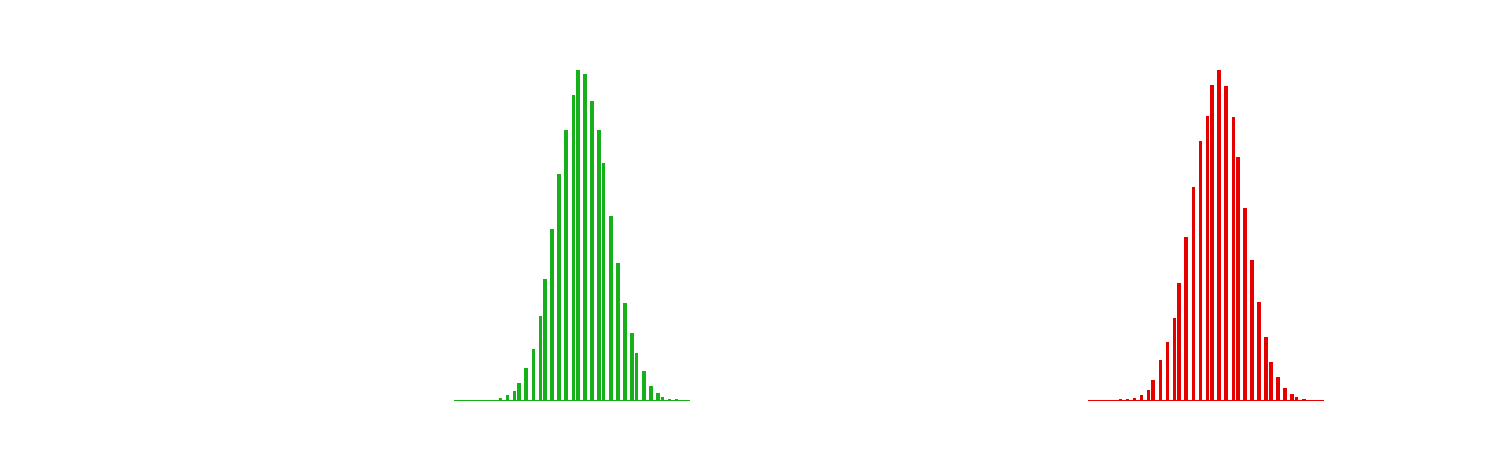
\includegraphics[width=\textwidth]{Results/3.5_boundariesBistability/maxReach0_0_HistogramPlot.pdf}
                    \label{}
                \end{minipage}
            \end{minipage}
            \begin{minipage}{0.77\textwidth}
                \begin{minipage}{0.1\textwidth}
                    \caption*{\small \textbf{(b)}}
                \end{minipage}
                \begin{minipage}{0.66\textwidth}
                    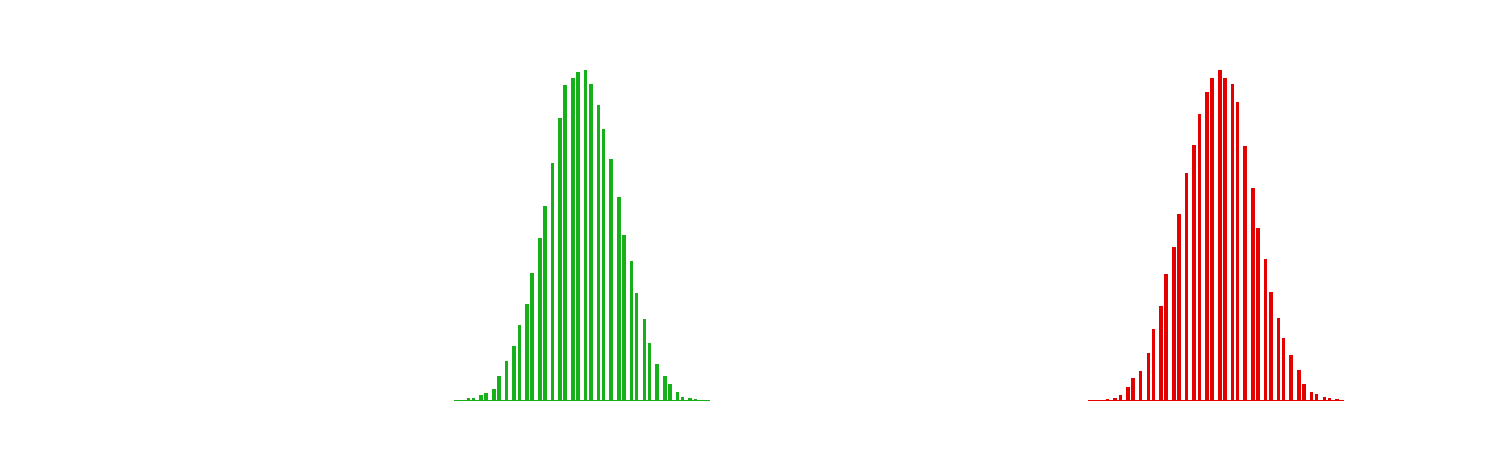
\includegraphics[width=\textwidth]{Results/3.5_boundariesBistability/maxReach1_4_HistogramPlot.pdf}
                \end{minipage}
            \end{minipage}
            \begin{minipage}{0.77\textwidth}
                \begin{minipage}{0.1\textwidth}
                    \caption*{\small \textbf{(c)}}
                    \label{}
                \end{minipage}
                \begin{minipage}{0.66\textwidth}
                    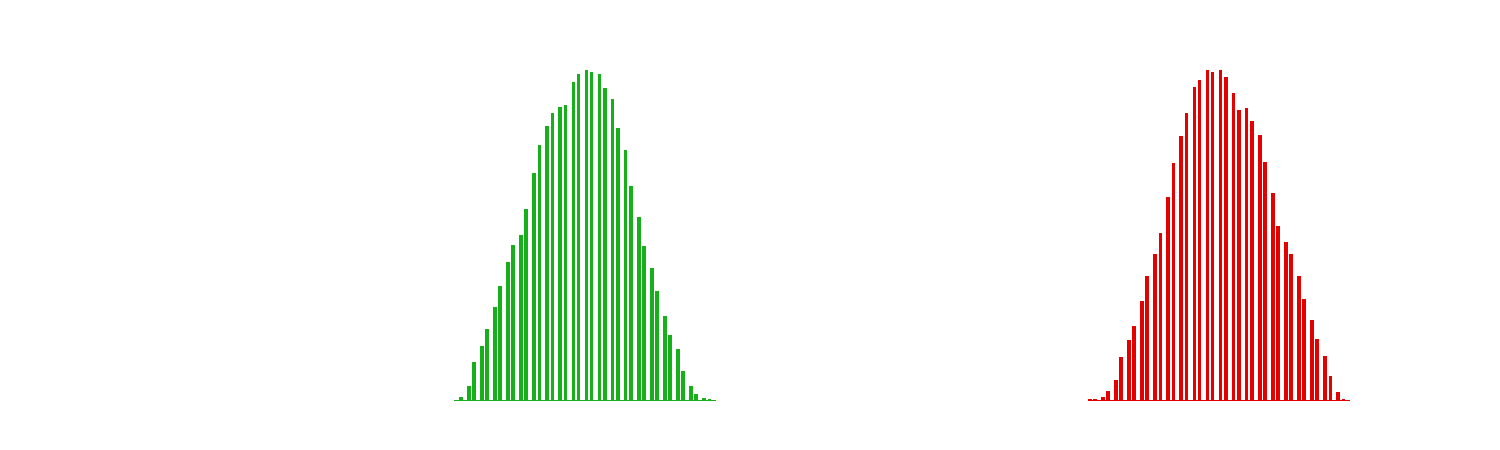
\includegraphics[width=\textwidth]{Results/3.5_boundariesBistability/maxReach2_2_HistogramPlot.pdf}
                    \label{}
                \end{minipage}
            \end{minipage}
            \begin{minipage}{0.77\textwidth}
                \begin{minipage}{0.1\textwidth}
                    \caption*{\small \textbf{(d)}}
                \end{minipage}
                \begin{minipage}{0.66\textwidth}
                    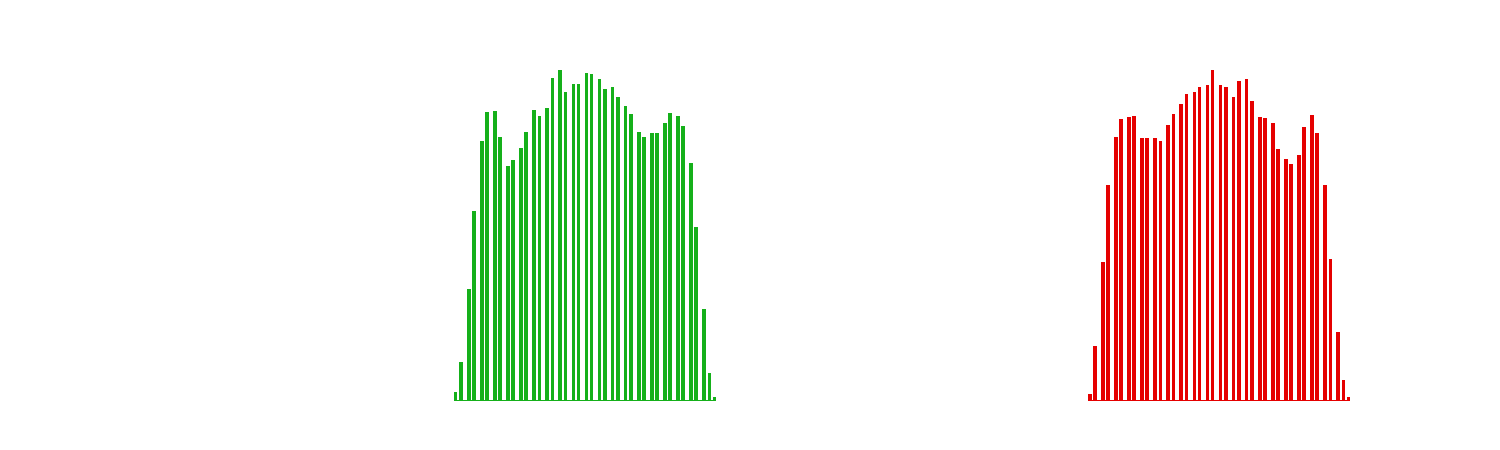
\includegraphics[width=\textwidth]{Results/3.5_boundariesBistability/maxReach3_3_HistogramPlot.pdf}
                \end{minipage}
            \end{minipage}
            \begin{minipage}{0.77\textwidth}
                \begin{minipage}{0.1\textwidth}
                    \caption*{\small \textbf{(e)}}
                    \label{}
                \end{minipage}
                \begin{minipage}{0.66\textwidth}
                    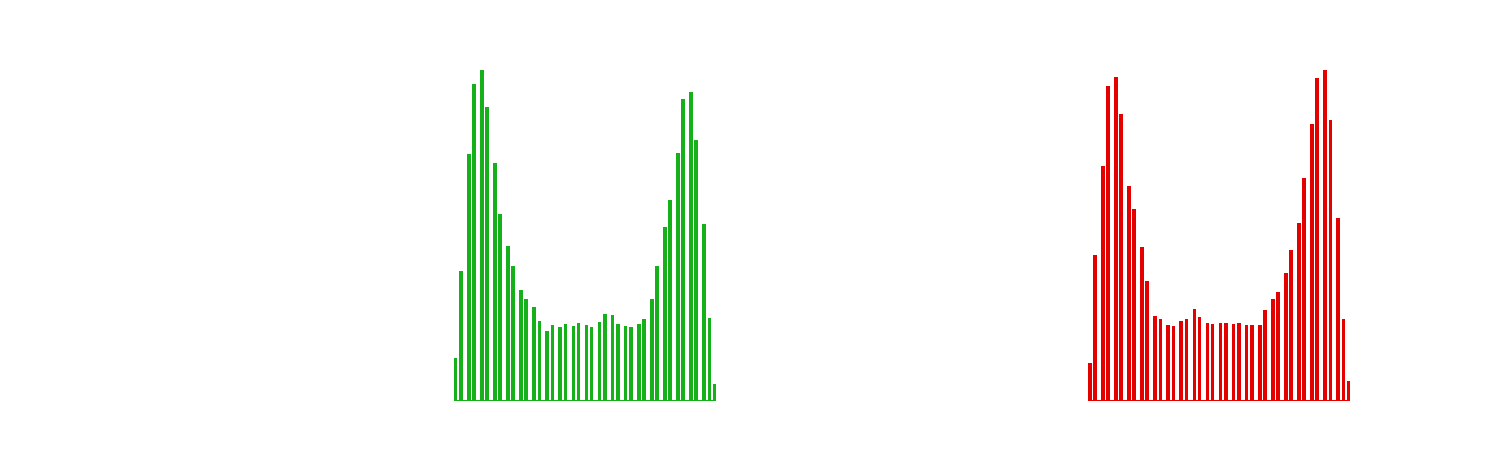
\includegraphics[width=\textwidth]{Results/3.5_boundariesBistability/maxReach4_3_HistogramPlot.pdf}
                    \label{}
                \end{minipage}
            \end{minipage}
            \begin{minipage}{0.77\textwidth}
                \begin{minipage}{0.1\textwidth}
                    \caption*{\small \textbf{(f)}}
                \end{minipage}
                \begin{minipage}{0.66\textwidth}
                    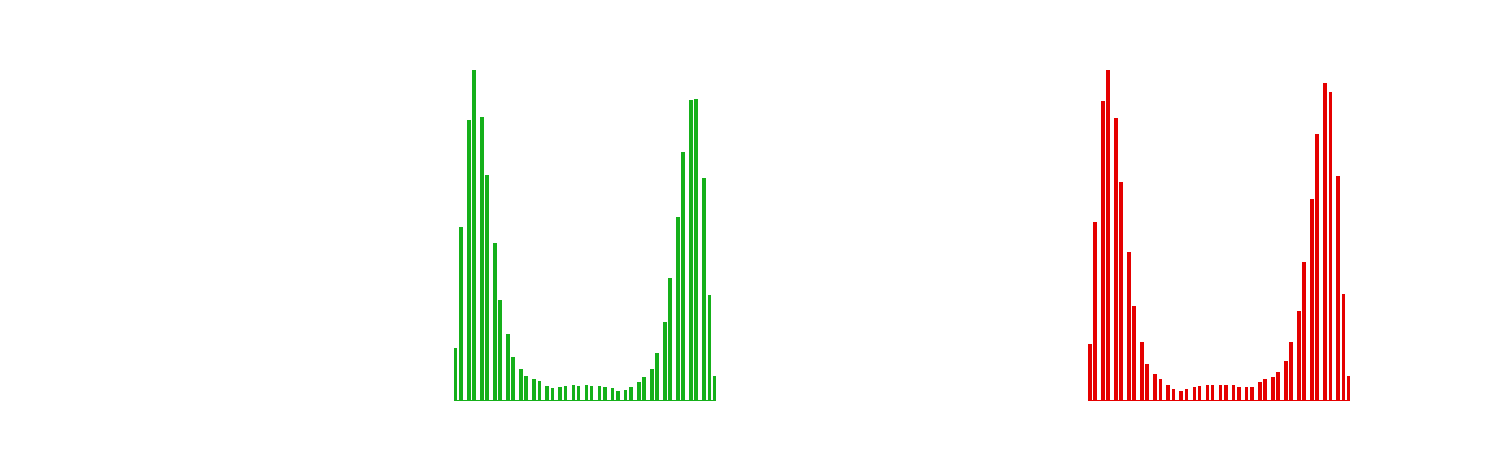
\includegraphics[width=\textwidth]{Results/3.5_boundariesBistability/maxReach5_4_HistogramPlot.pdf}
                \end{minipage}
            \end{minipage}
            \begin{minipage}{0.77\textwidth}
                \begin{minipage}{0.1\textwidth}
                    \caption*{\small \textbf{(g)}}
                \end{minipage}
                \begin{minipage}{0.66\textwidth}
                    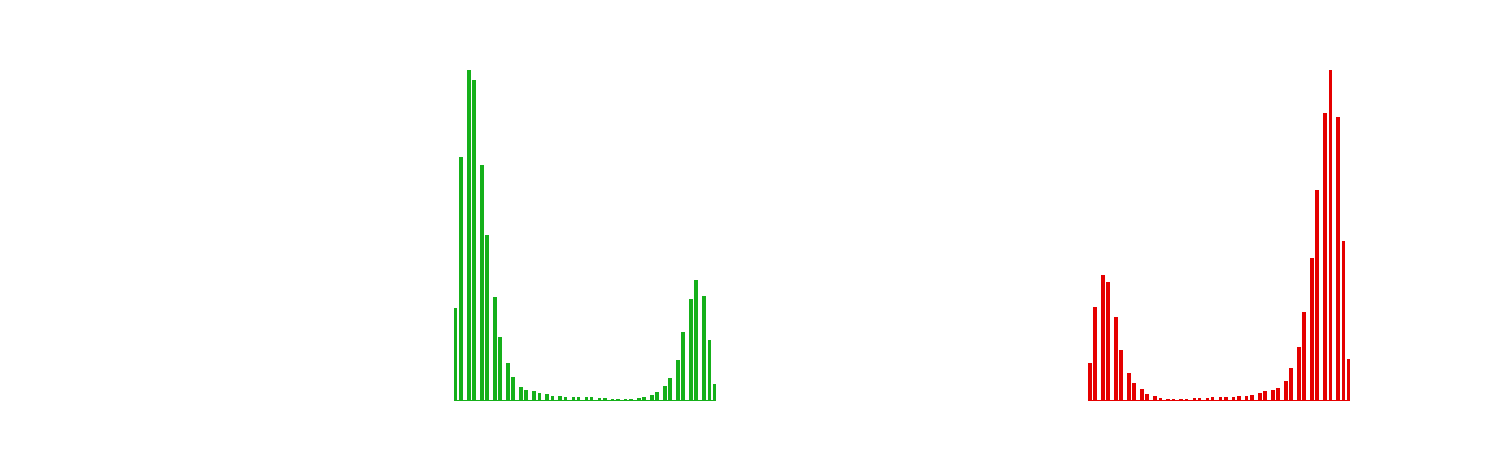
\includegraphics[width=\textwidth]{Results/3.5_boundariesBistability/maxReach6_4_HistogramPlot.pdf}
                \end{minipage}
            \end{minipage}
            \caption{Graphical depiction of the possible cooperative enzyme acetylation addition \textbf{(a)} and removal \textbf{(b)} reactions. The reactions shown are also defined in the rule set to occur in the opposite direction. Cooperative enzyme methylators work analogically.}
            \label{img:linearEnzyme}
        \end{figure}
        %
        \begin{itemize}
            {
                \color{red}
                \item describe loss of reach
                \item run without unmodified state?
            }
        \end{itemize}
        %
    %
    %
    \newpage
    \section{Bivalency} % TODO Should I include these  cases into the others above? Pro: I don't find anything ground-breaking here. Con: I have an entirely different system which might lead to confusion
        \label{sec:ResBivalency}
        %
        \begin{itemize}
            {
                \color{red}
                \item Here, we are at Kx+Ky
                \item Two systems that either favour bivalency or total active/silent states as an introduction to bivalency
                \item Frequent switching and bivalency
            }
        \end{itemize}
        %
    %
    %
%
%